\documentclass{standalone}

\usepackage[latin1]{inputenc}
\usepackage{amsmath}
\usepackage{amssymb}
\usepackage{amsthm}

\usepackage{tikz}
\usetikzlibrary{arrows}
%\usetikzlibrary{calc}
%\usetikzlibrary{snakes}

%% generates a tightly fitting border around the work
%\usepackage[active,tightpage]{preview}
%\PreviewEnvironment{tikzpicture}
%\setlength\PreviewBorder{0.5mm}
%%\renewcommand\PreviewBbAdjust{-\PreviewBorder 1mm -1.15mm -0.85mm}

\usepackage{color}

%\pagestyle{empty}

\begin{document}

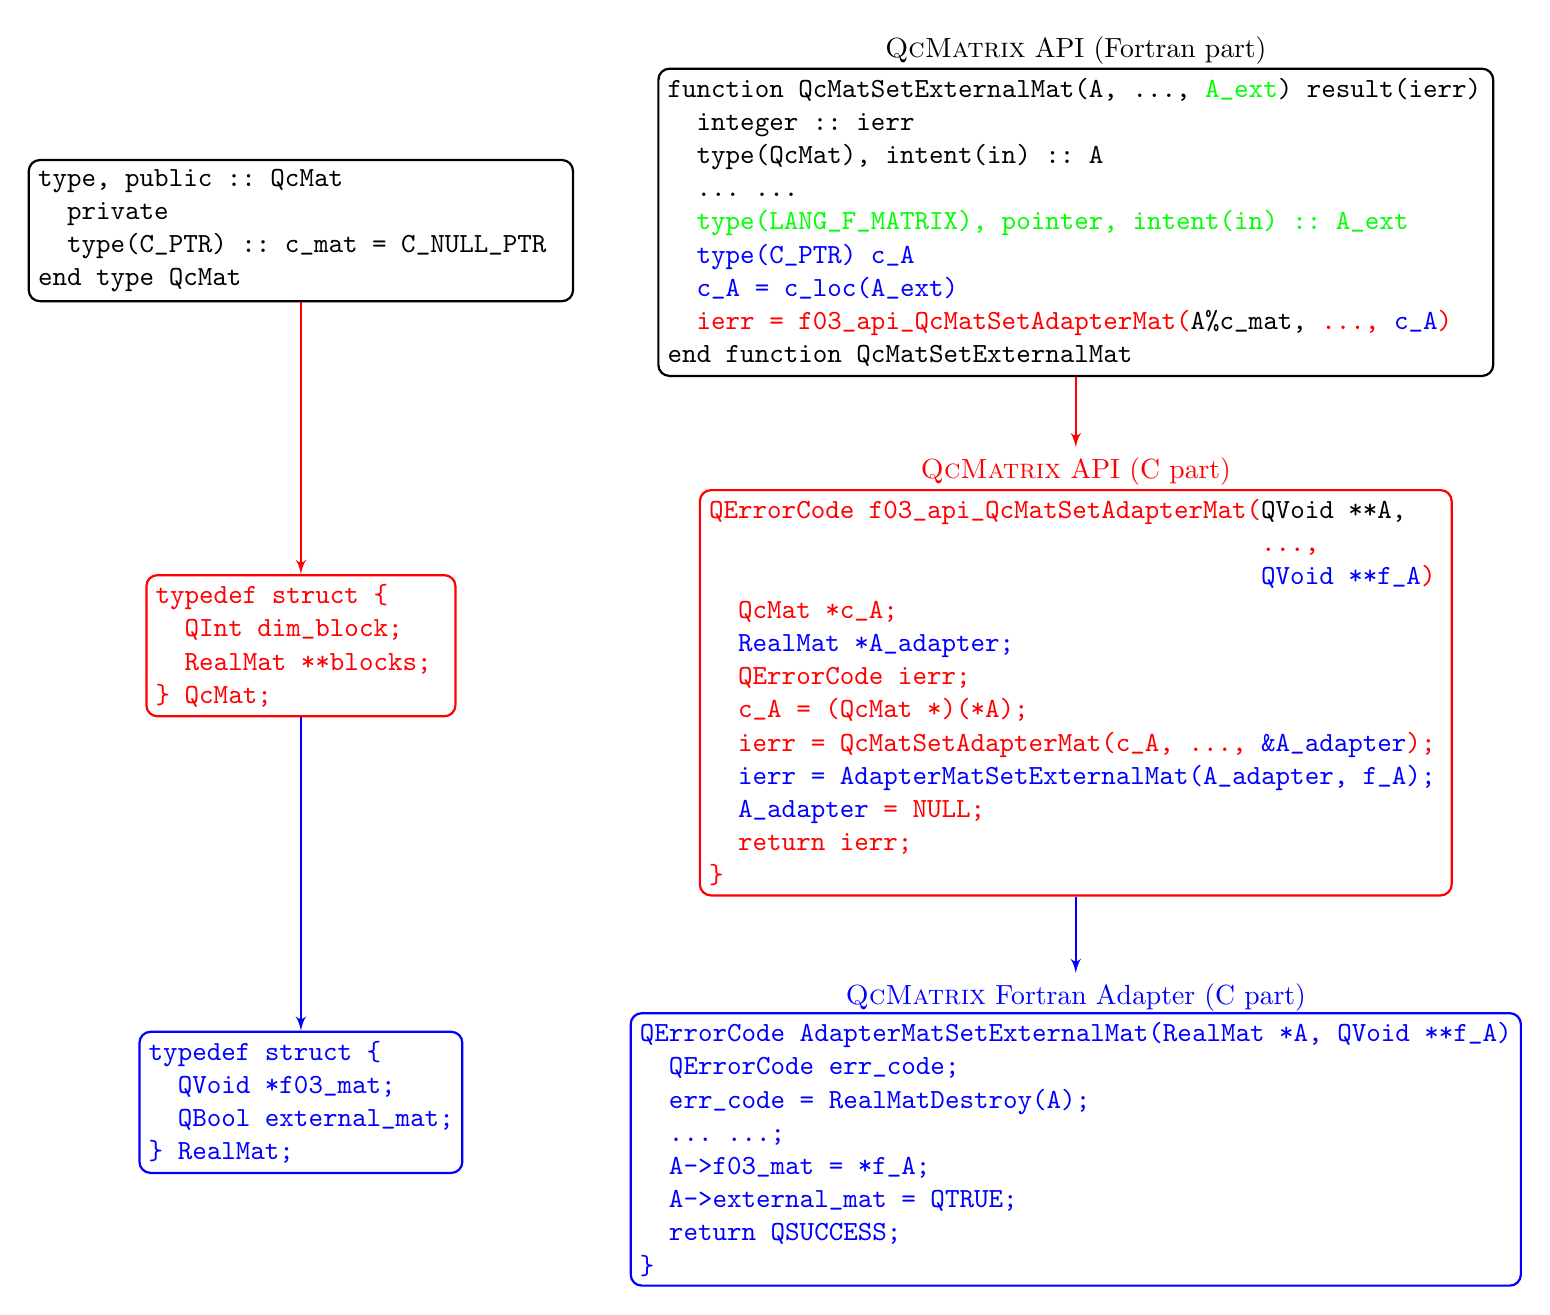
\begin{tikzpicture}[thick]
  % QcMat (Fortran)
  \node[color=black, rectangle, draw, text badly ragged, rounded corners, %
        minimum height=20, text width=190] (QcMatFDef) %
       {\verb|type, public :: QcMat| %
        \linebreak\verb|  private| %
        \linebreak\verb|  type(C_PTR) :: c_mat = C_NULL_PTR|
        \linebreak\verb|end type QcMat|};
  % QcMat
  \node[color=red, rectangle, draw, text badly ragged, rounded corners, %
        minimum height=20, text width=105, below of=QcMatFDef, node distance=150] (QcMatDef) %
       {\verb|typedef struct {| %
        \linebreak\verb|  QInt dim_block;| %
        \linebreak\verb|  RealMat **blocks;| %
        \linebreak\verb|} QcMat;|};
  \draw [color=red, -latex'] (QcMatFDef)--(QcMatDef);
  % RealMat
  \node[color=blue, rectangle, draw, text badly ragged, rounded corners, minimum height=20,
        text width=110, below of=QcMatDef, node distance=165] (RealMatDef) %
       {\verb|typedef struct {| %
        \linebreak\verb|  QVoid *f03_mat;| %
        \linebreak\verb|  QBool external_mat;| %
        \linebreak\verb|} RealMat;|};
  \draw [color=blue, -latex'] (QcMatDef)--(RealMatDef);
  % APIs
  \node[color=black, right of=QcMatFDef, node distance=280, yshift=65] (NoteAPIF) %
       {\textsc{QcMatrix} API (Fortran part)};
  \node[color=black, rectangle, draw, text badly ragged, rounded corners, minimum height=20, % 
        text width=295, below of=NoteAPIF, node distance=62] (APIF) %
       {\verb|function QcMatSetExternalMat(A, ..., |\color{green}\verb|A_ext|\color{black}\verb|) result(ierr)| %
        \linebreak\verb|  integer :: ierr| %
        \linebreak\verb|  type(QcMat), intent(in) :: A| %
        \linebreak\verb|  ... ...| %
        \linebreak\color{green}\verb|  type(LANG_F_MATRIX), pointer, intent(in) :: A_ext| %
        \linebreak\color{blue}\verb|  type(C_PTR) c_A| %
        \linebreak\color{blue}\verb|  c_A = c_loc(A_ext)| %
        \linebreak\color{red}\verb|  ierr = f03_api_QcMatSetAdapterMat(|\color{black}\verb|A%c_mat, |\color{red}\verb|..., |\color{blue}\verb|c_A|\color{red}\verb|)| %
        \linebreak\color{black}\verb|end function QcMatSetExternalMat|};
  \node[color=red, below of=APIF, node distance=90] (NoteAPIC) {\textsc{QcMatrix} API (C part)};
  \node[color=red, rectangle, draw, text badly ragged, rounded corners, minimum height=20, % 
        text width=265, below of=NoteAPIC, node distance=80] (APIC) %
       {\verb|QErrorCode f03_api_QcMatSetAdapterMat(|\color{black}\verb|QVoid **A,| %
        \linebreak\color{red}\verb|                                      ...,| %
        \linebreak\color{blue}\verb|                                      QVoid **f_A|\color{red}\verb|)| %
        \linebreak\verb|  QcMat *c_A;| %
        \linebreak\color{blue}\verb|  RealMat *A_adapter;| %
        \linebreak\color{red}\verb|  QErrorCode ierr;| %
        \linebreak\verb|  c_A = (QcMat *)(*A);| %
        \linebreak\verb|  ierr = QcMatSetAdapterMat(c_A, ..., |\color{blue}\verb|&A_adapter|\color{red}\verb|);| %
        \linebreak\color{blue}\verb|  ierr = AdapterMatSetExternalMat(A_adapter, f_A);| %
        \linebreak\verb|  A_adapter|\color{red}\verb| = NULL;| %
        \linebreak\verb|  return ierr;| %
        \linebreak\verb|}|};
  \draw [color=red, -latex'] (APIF)--(NoteAPIC);
  % adapater
  \node[color=blue, below of=APIC, node distance=110] (NoteAdapterC) %
       {\textsc{QcMatrix} Fortran Adapter (C part)};
  \node[color=blue, rectangle, draw, text badly ragged, rounded corners, minimum height=20, % 
        text width=315, below of=NoteAdapterC, node distance=55] (AdapterC) %
       {\verb|QErrorCode AdapterMatSetExternalMat(RealMat *A, QVoid **f_A)| %
        \linebreak\verb|  QErrorCode err_code;| %
        \linebreak\verb|  err_code = RealMatDestroy(A);| %
        \linebreak\verb|  ... ...;| %
        \linebreak\verb|  A->f03_mat = *f_A;| %
        \linebreak\verb|  A->external_mat = QTRUE;| %
        \linebreak\verb|  return QSUCCESS;| %
        \linebreak\verb|}|};
  \draw [color=blue, -latex'] (APIC)--(NoteAdapterC);
\end{tikzpicture}

\end{document}
